\documentclass[../main/thesis.tex]{subfiles}
\begin{document}

\chapter{3DMiMic I-V Measurements}
\label{a-iv}

\begin{figure}[h]
	\centering
	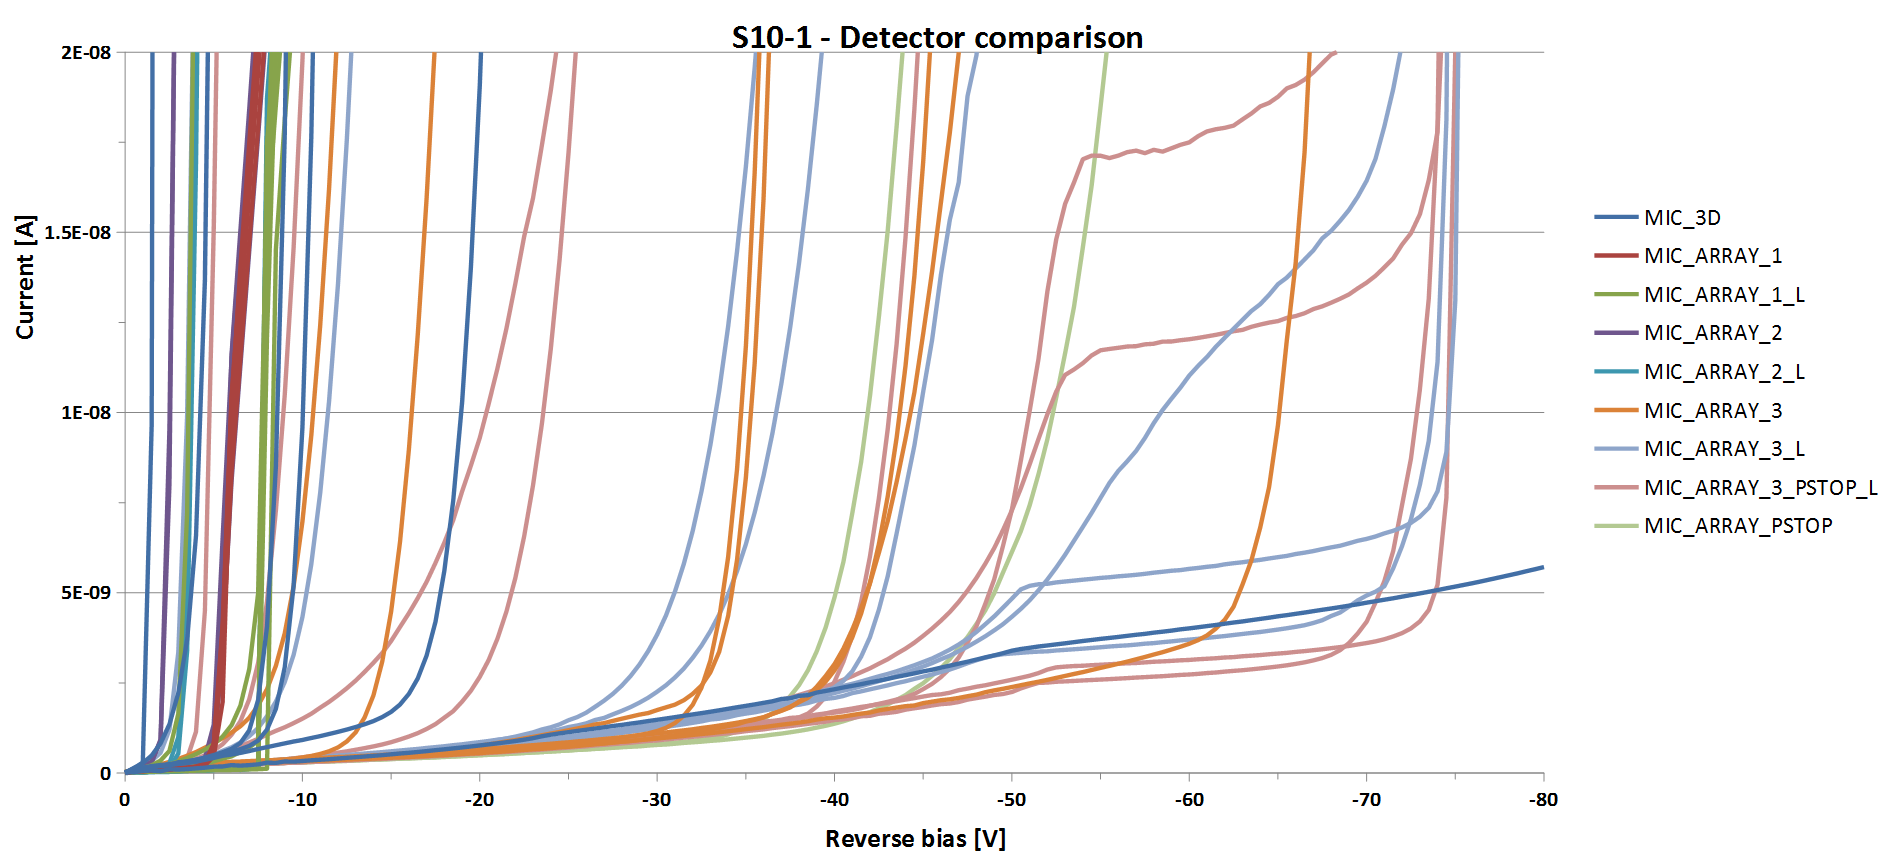
\includegraphics[width=0.9\textwidth]{S10-1.png}
	\caption{I-V measurement of the S10-1 wafer. }
	\label{fig-3d-S10-1} 
\end{figure}

\begin{figure}[b!]
	\centering
	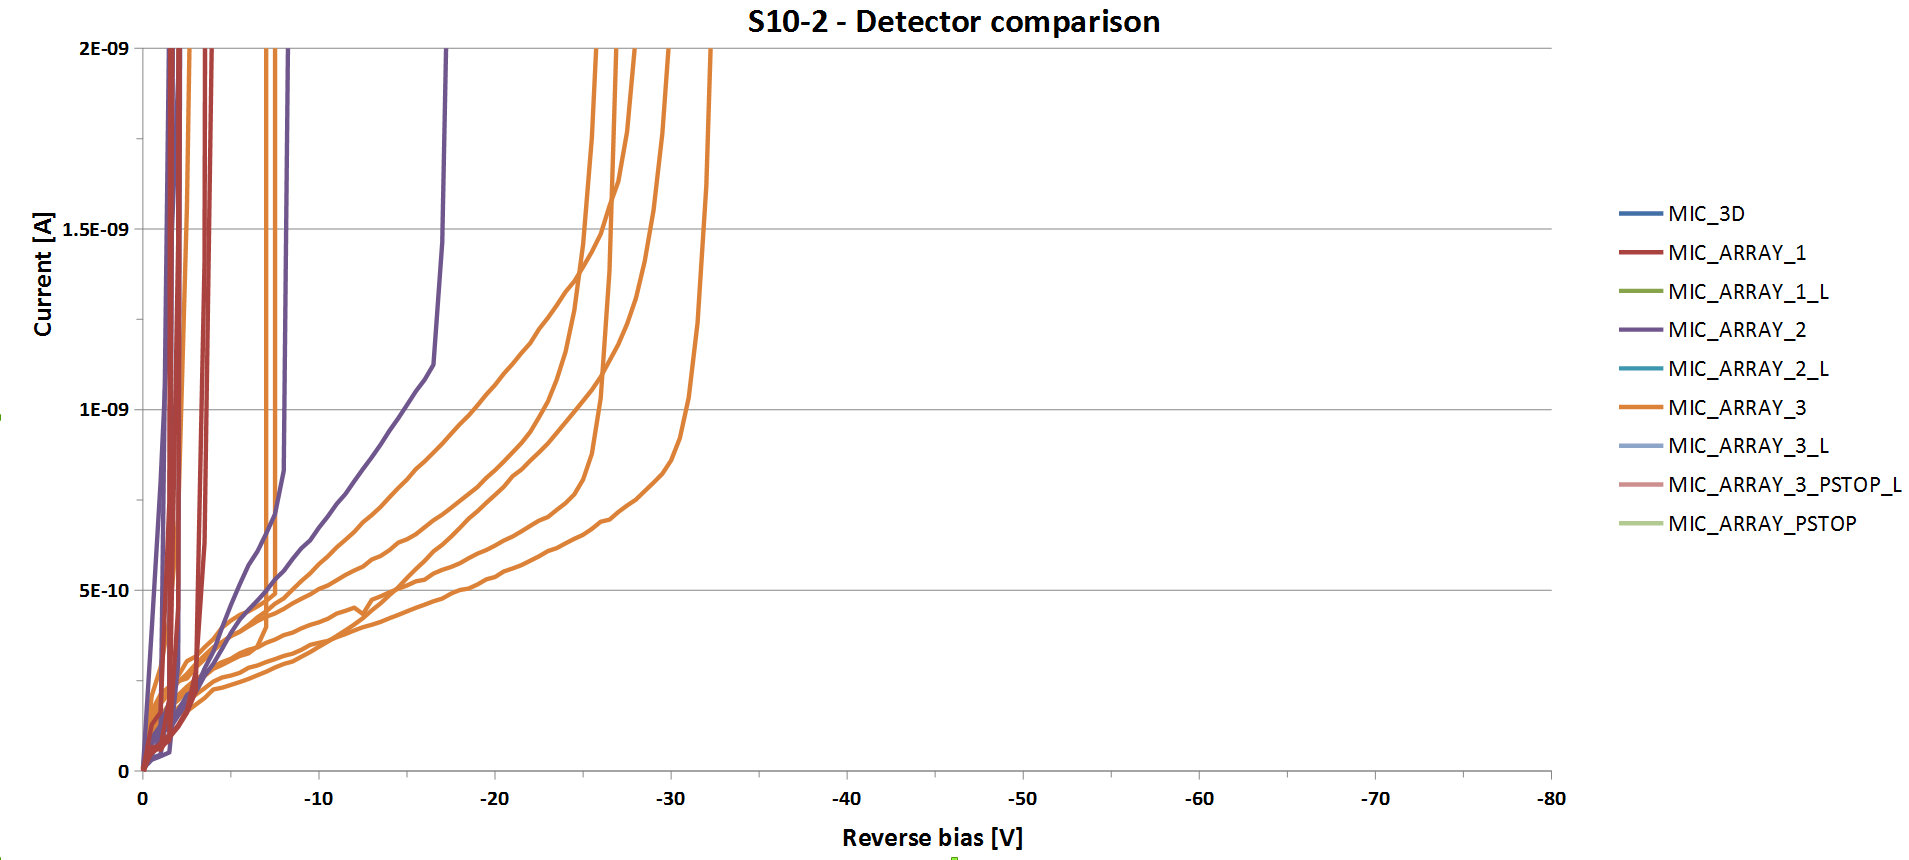
\includegraphics[width=0.9\textwidth]{S10-2.png}
	\caption{I-V measurement of the S10-2 wafer. }
	\label{fig-3d-S10-2} 
\end{figure}

\begin{figure}%[h]
	\centering
	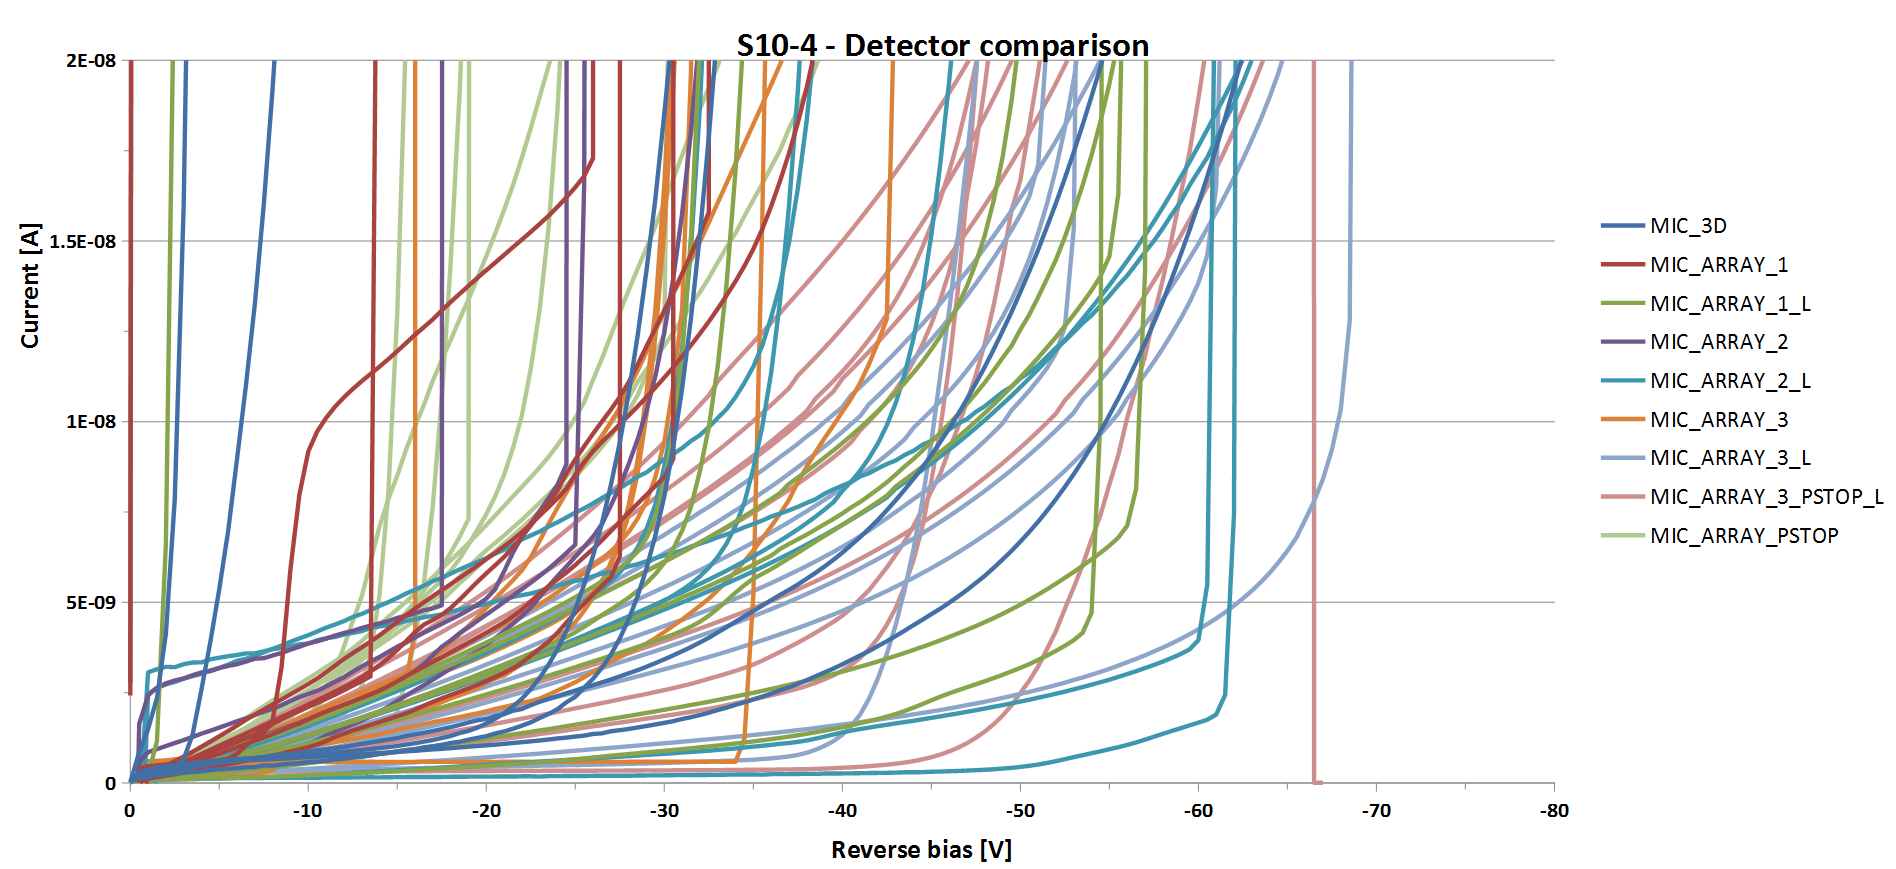
\includegraphics[width=0.9\textwidth]{S10-4.png}
	\caption{I-V measurement of the S10-4 wafer. }
	\label{fig-3d-S10-4} 
\end{figure}

\begin{figure}%[h]
	\centering
	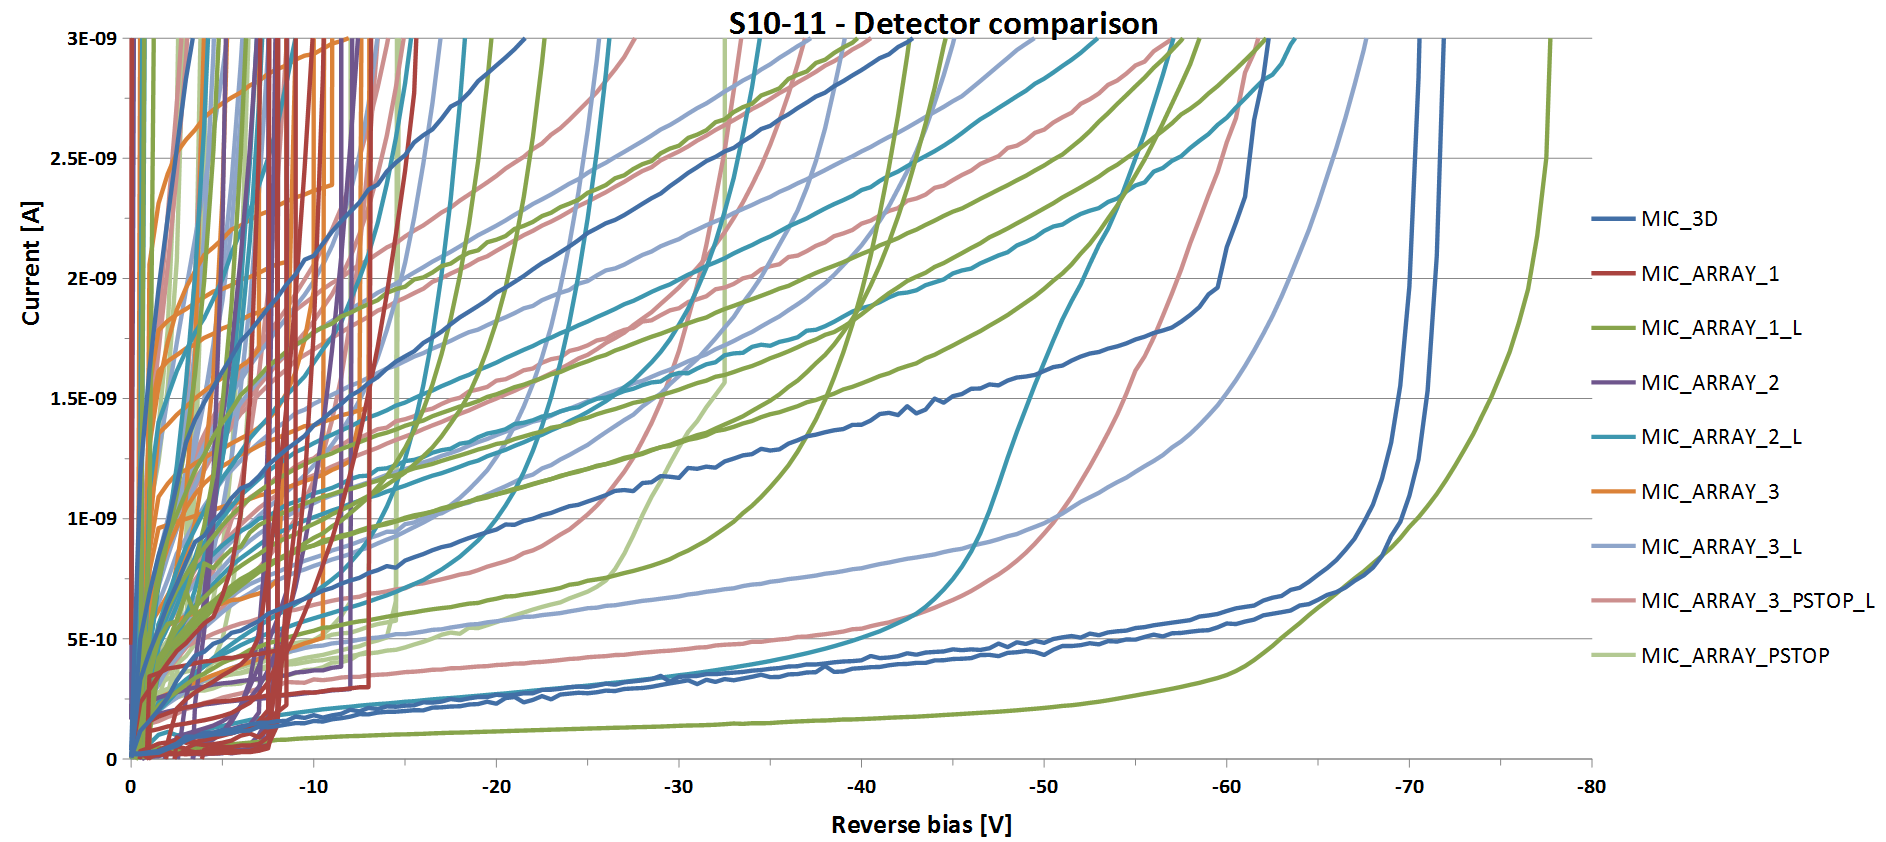
\includegraphics[width=0.9\textwidth]{S10-11.png}
	\caption{I-V measurement of the S10-11 wafer. }
	\label{fig-3d-S10-11} 
\end{figure}

\begin{figure}%[h]
	\centering
	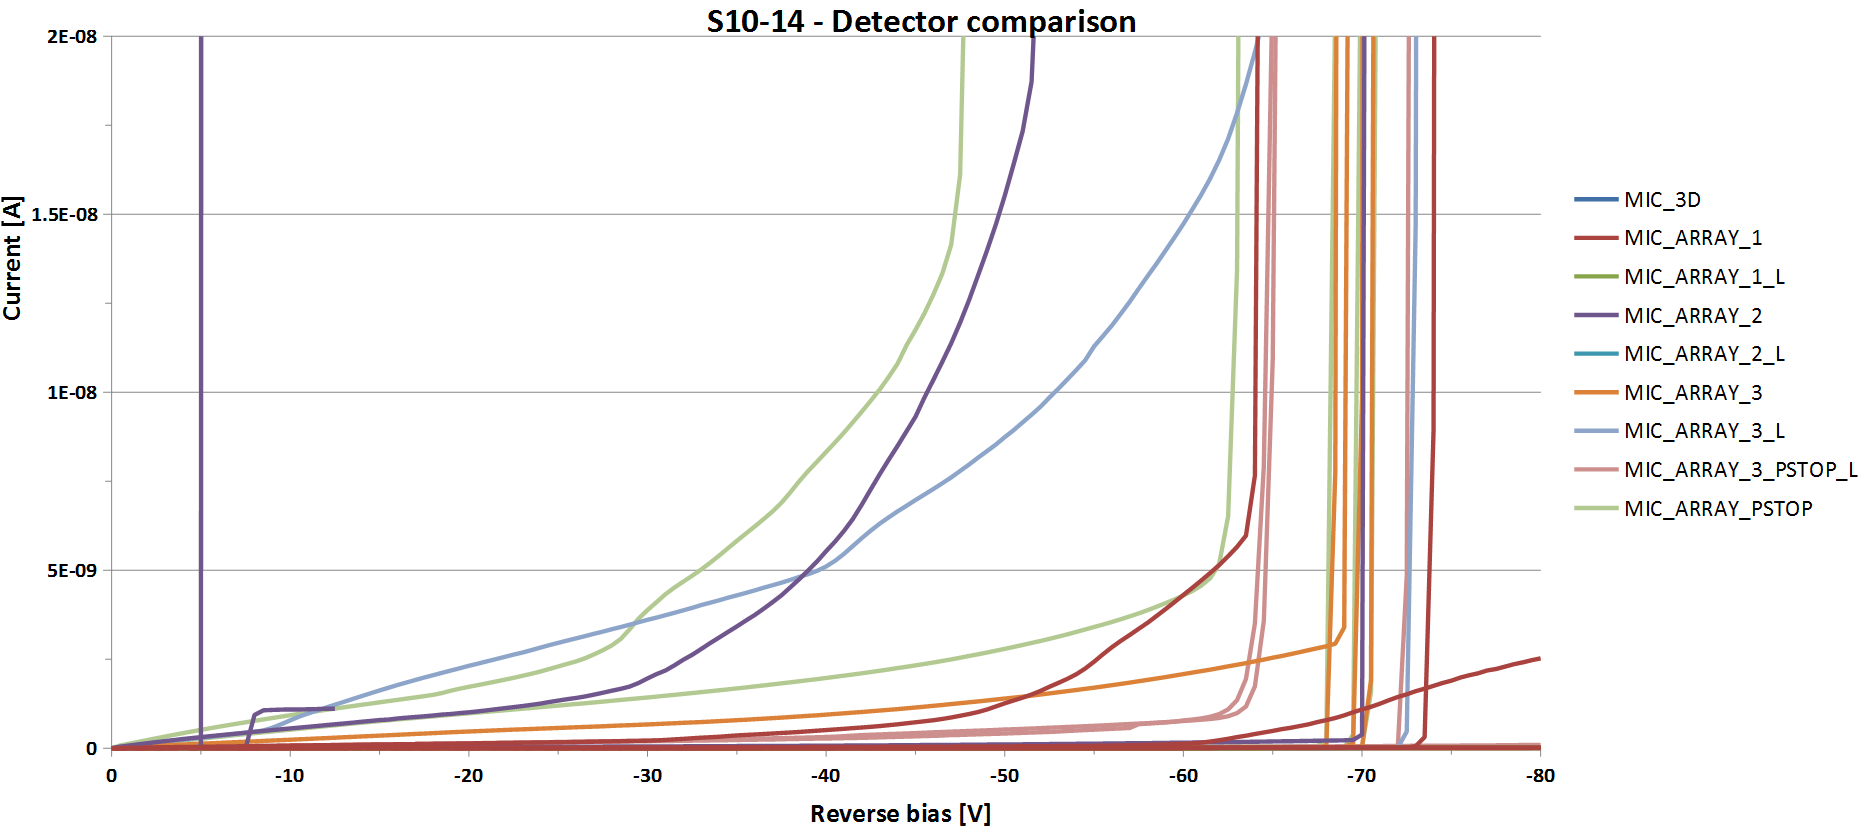
\includegraphics[width=0.9\textwidth]{S10-14.png}
	\caption{I-V measurement of the S10-14 wafer. }
	\label{fig-3d-S10-14} 
\end{figure}

\begin{figure}%[h]
	\centering
	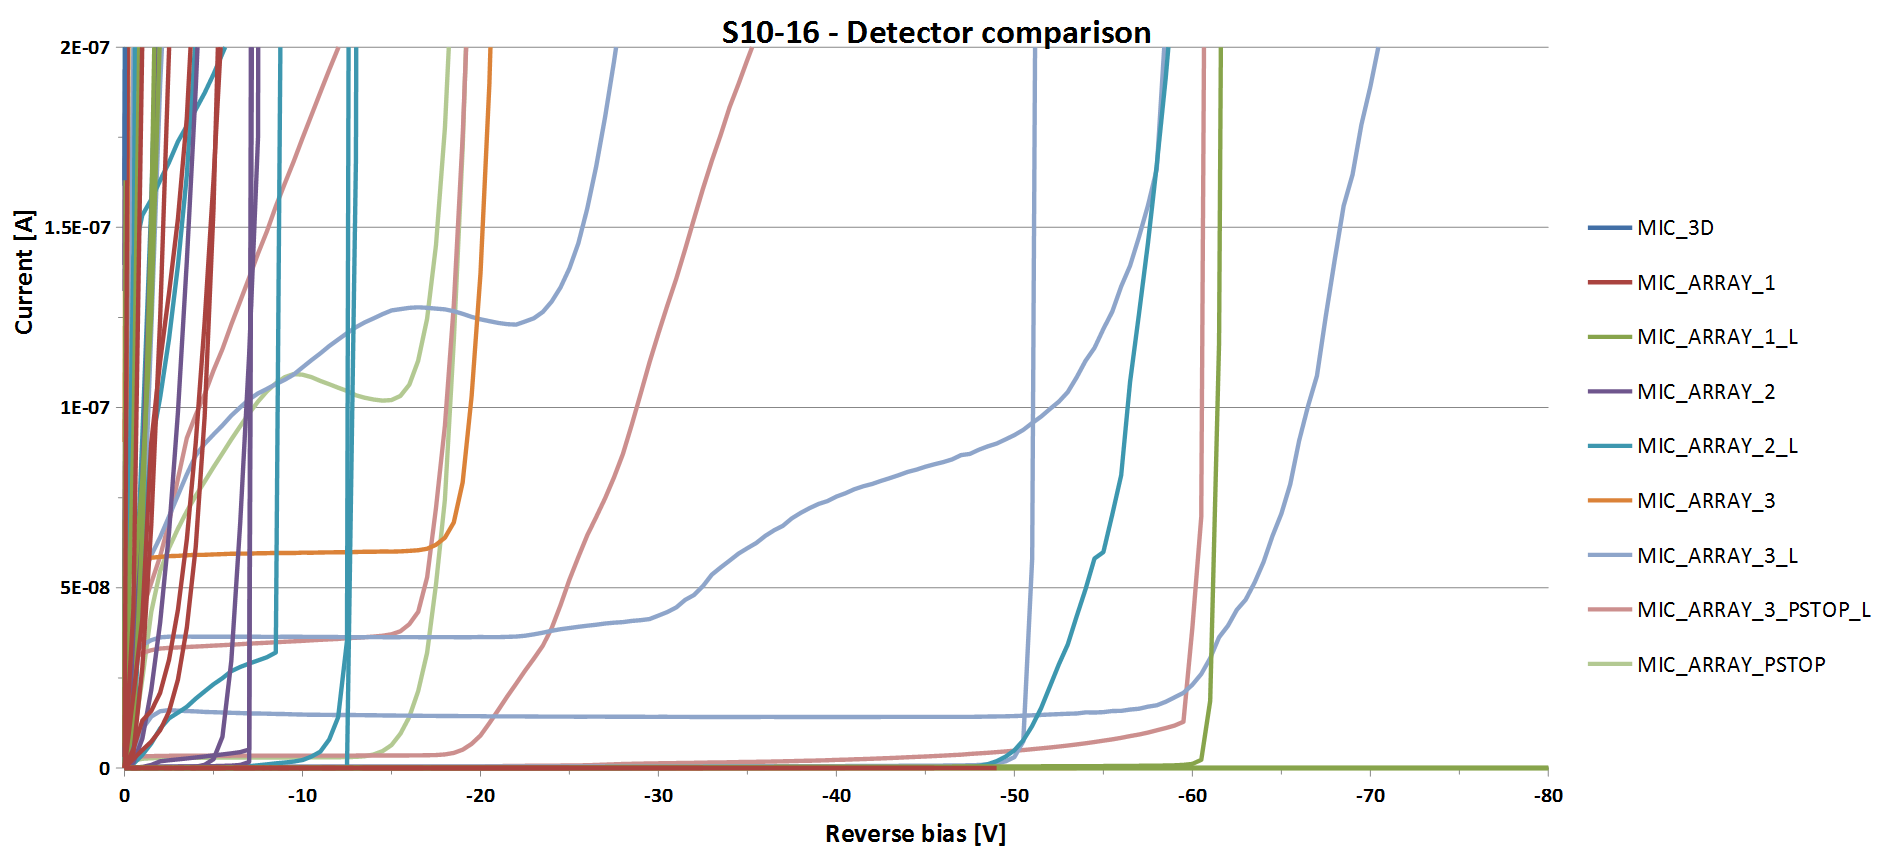
\includegraphics[width=0.9\textwidth]{S10-16.png}
	\caption{I-V measurement of the S10-16 wafer. }
	\label{fig-3d-S10-16} 
\end{figure}

\begin{figure}%[h]
	\centering
	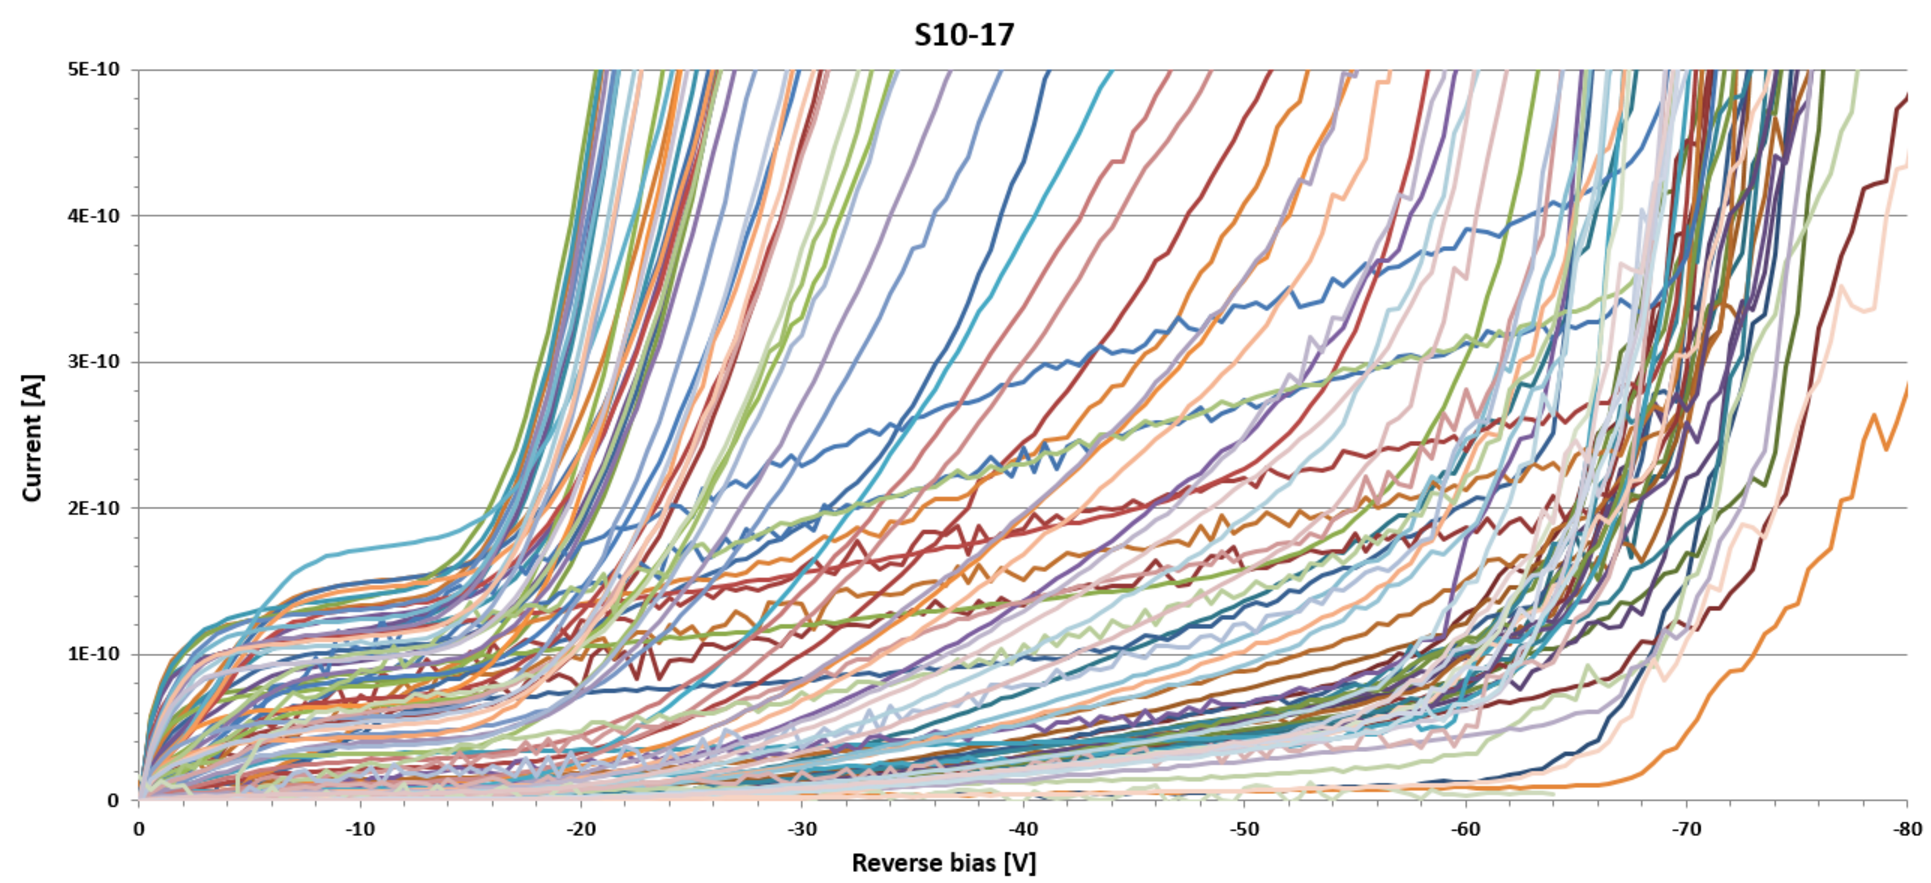
\includegraphics[width=0.9\textwidth]{S10-17.png}
	\caption{I-V measurement of the S10-17 wafer. }
	\label{fig-3d-S10-17-} 
\end{figure}

\end{document}